\chapter{CNT}
Taken from OnlineMathCircle lecture 4.

In this lecture we'll develop some common problem-solving techniques in combinatorics, and see how they apply to problems with a number theoretic flavor. Finally, we'll prove some classic theorems in combinatorial number theory such as the Cauchy-Davenport Theorem on additive sets modulo $p$ and Van der Waerden's Theorem on monochromatic arithmetic progressions.
\section{Pigeonhole Principle}
The Pigeonhole Principle will be our first main strategy.
\begin{thm}[Pigeonhole/Box Principle]
Suppose there are more than $kn$ objects divided into $n$ categories. Then some category must have more than $k$ objects.
\end{thm}
\begin{proof}
If all of the categories have at most $k$ objects, then there can only be at most $kn$ objects. 
\end{proof}
Think of the objects as pigeons and the categories as holes.

\begin{figure}[h!]
\centering
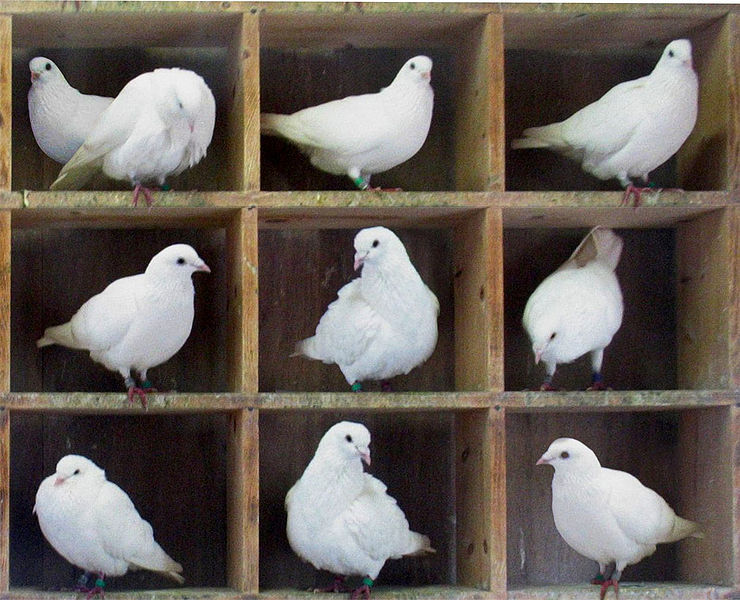
\includegraphics[scale=0.5]{cnt-chapters/toomanypigeons}
\caption{From http://en.wikipedia.org/wiki/File:TooManyPigeons.jpg}
\end{figure}

There are two basic questions to ask when applying the pigeonhole principle:
\begin{enumerate}
\item
What are the pigeons?
\item
What are the holes?
\end{enumerate}
Often the solution to a difficult problem hinges on the correct answer to these two questions; sometimes the pigeons and boxes have to be chosen in creative ways!
\begin{ex}
Let $A$ be a set of $n$ integers. Prove that $A$ contains a subset such that the sum of its elements is divisible by $n$.
\end{ex}
\begin{proof}
Label the elements of $A$ as $a_1,\ldots,a_n$.  
Define the partial sums
\begin{align*}
s_0&=0\\
s_1&=a_1\\
s_2&=a_1+a_2\\
\vdots&\;\;\;\;\;\vdots\\
s_n&=a_1+a_2+ \cdots+a_n.
\end{align*}
Since there are $n+1$ numbers and $n$ possible residues modulo $n$, by the Pigeonhole Principle two of them, say $s_i$ and $s_j$, have the same residue modulo $n$. Suppose without loss of generality that $i<j$. Then 
\[s_j-s_i=a_{i+1}+\cdots +a_j\]
is divisible by $n$, as needed.

Here the pigeons are the partial sums, and the holes are the residues modulo $n$. Note that we considered the partial sums, so that the difference of two of them is a sum of elements of $A$. 
\end{proof}
\begin{thm}[Dirichlet/Kronecker] Let $a$ be a real number and $\ep>0$. Then there exists a positive integer $p$ and an integer $m$ such that $\left|pa-m\right|< \ep$.
\end{thm}
In other words, given any number, we can find a multiple of it that is as close to an integer as we want.
\begin{proof}
Equivalently, we want to find $p$ such that $\{pa\}$ is either in $[0,\ep)$ or $(1-\ep,1)$, because then we could either set $m=\fl{pa}$, ($pa$ rounded down to the nearest integer) or $m=\ce{pa}$ ($pa$ rounded up to the nearest integer). Hence we just focus on the fractional parts of the multiples of $a$. We note that if $\{pa\}$ and $\{qa\}$ are close together, then $|p-q|a$ will be close to an integer. We make this precise below. 

Choose an integer $N$ such that $N\ge\rc{\ep}$. 
The elements $\{pa\}$ for $1\leq p\leq N+1$ fall in one of the $N$ intervals
\[\left[\frac{0}{N},\frac{1}{N}\right),\left[\frac{1}{N},\frac{2}{N} \right),\ldots, \left[\frac{N-1}{N},\frac{N}{N}\right).\]
By the Pigeonhole Principle, two of the $\{p\al\}$ fall in the same interval, say $p\al$ and $q\al$. Then 
$\{|p-q|\al\}\in \left[ 0,\rc{N}\right) \cup \left(\frac{N-1}{N},1\right)
\subeq[0,\ep)\cup(1-\ep,1)
,$
as needed.

In this problem the pigeons are the fractional parts and the holes are the intervals above.
\end{proof}
\begin{rem}
The above proof shows that one of the numbers $a,\ldots, Na$ is at most a distance of $\rc{N}$ away from an integer. Can you show that in fact one of the numbers $a,\ldots, (N-1)a$ is at most at distance of $\rc{N}$ from an integer?
\end{rem} 
%\pagebreak
{\Large Problems 1}
\begin{enumerate}
\item Prove that if one chooses more than $n$ numbers from the set
$\{1,2,3,...,2n\}$, then 
\begin{enumerate}
\item two of them are relatively prime, and 
\item one number is a multiple of another.
\end{enumerate}
\item Prove that for every $n$, there is a nonzero Fibonacci number divisible by $n$. (The Fibonacci numbers are defined by $F_0=0, F_1=1$ and $F_{n+2}=F_{n+1}+F_n$.)
\item A set $S$ of distinct integers each of which is greater than or equal to 1 and less than or equal to $n$ is given. 
\begin{enumerate}
\item If $S$ consists of $\fl{\frac n2}+1$ elements, is it possible that no element of $S$ is the sum of two \textbf{distinct} elements of $S$? 
\item If $S$ consists of $\fl{\frac n2}+2$ elements, prove that the largest element of $S$ is the sum of 2 distinct elements of $S$ and the smallest element is the difference of two distinct elements of $S$. 
\item 
Find the smallest positive integer $m$ (in terms of $n$) such that if $S$ has $m$ elements, then some element of $S$ is the sum of 3 distinct elements of $S$.
\end{enumerate}
\item Prove that any subset of $\{1,\ldots, n\}$ with at least $\fl{\frac{n+k}{2}}+1$ elements contains two elements differing by $k$.
\item (Putnam 2006/B2) Prove that for every set $X=\{x_1,\ldots, x_n\}$ of real numbers, there exists a non-empty subset $S$ of $X$ and an integer $m$ such that 
\[\ab{m+\sum_{s\in S} s}\leq \rc{n+1}.\]
\item (IMO 1972/1) Let $S$ be a set of 10 arbitrary 2-digit numbers. Prove that one can
find two disjoint subsets of $S$ with the same sum of elements.
\item (Romania) Find the greatest positive integer $n$ with the following property:
there exist $n$ nonnegative integers $x_{1},x_{2},\ldots,x_{n}$, at least one
different from zero, such that for any numbers $a_{1},a_{2},\ldots,a_{n}
\in\left\{  -1,0,1\right\}$, at least one different from zero, $n^{3}$ does
not divide $a_{1}x_{1}+a_{2}x_{2}+\ldots+a_{n}x_{n}$.
\item Given 25 positive integers all of whose prime factors are in the set $\{2,3,5\}$, prove that there are 4 numbers whose product is the 4th power of an integer.
\item Let $a_1,\ldots, a_n$ be real numbers. Show that for any $\ep>0$ there exists a positive integer $p$ and integers $m_i$ so that
\[|pa_i-m_i|<\ep\]
for all $i$. 
\item For a positive real number $a$, let $S_a=\{\fl{na}|n\in \N\}$. Do there exist $a,b,c$ such that $S_a,S_b$, and $S_c$ are disjoint? (Hint: Use the previous problem.)
\item Let $S$ be a set of $n$ positive integers, and let $m$ be a positive integer. Prove that there are at least $2^{n-m+1}$ subsets of $S$ with sum of elements divisible by $m$. Include the empty set in your count. 
\item (Romania 1996) Let $n$ be an integer greater than 2 and let $S$ be a $3n^2$ - element subset of the set $\left\{1,2,\ldots,n^3\right\}$. Prove that one can find nine distinct numbers $a_{1},a_{2},\ldots,a_{9}$ in $S$ such that the system
\begin{align*}
a_{1}x+a_{2}y+a_{3}z&=0\\
a_{4}x+a_{5}y+a_{6}z&=0\\
a_{7}x+a_{8}y+a_{9}z&=0
\end{align*}
has a solution $(x_{0},y_{0},z_{0})$ in nonzero integers.

\item (\cite[\S 7.4]{Nat}) Let $A$ be a subset of the nonnegative integers $\N_0$ containing 0. Let $A(n)$ denote the number of nonzero elements of $A$ that are at most $n$, i.e. $A(n)=|A\cap [1,n]|$. Define the \textbf{Shnirel'man density} of $A$ to be{\footnote{The {\it infimum} of a set is like the minimum of the set. It is defined as the greatest lower bound for the set, so unlike the minimum it is always defined. For example, the infimum of the set $S=\{x|x>0\}$ is 0; however the minimum does not exist, because 0 is not in the set itself.}}
\[
\sigma(A)=\inf_{n\geq 1} \frac{A(n)}{n}.
\]
For two sets $A,B$, define the sumset to be all possible sums of an element in $A$ and an element in $B$:
\[
A+B=\{a+b\mid a\in A,b\in B\}.
\]
(The difference $A-B$ is defined similarly.) Define
\[
nA=\underbrace{A+\cdots +A}_n,
\]
i.e. $nA$ consists of numbers that are the sum of $n$ elements of $A$. We say that $A$ is a \textbf{basis} of order $n$ if $nA=\N_0$. 
Prove the following:
\begin{thm}[Shnirel'man] 
If $\sigma(A)>0$ then $A$ is a basis of finite order.
\end{thm}
Hints:
\begin{enumerate}
\item
Show that if $\sigma(A)+\sigma(B)\geq 1$, then $A+B=\N_0$. Conclude that if $\sigma(A)\geq \rc 2$, then $A$ is a basis of order 2. 
\item 
Prove that $\sigma(A+B)\geq \sigma(A)+\sigma(B)-\sigma(A)\sigma(B)$. (Note: it is true, although harder to prove, that $\sigma(A+B)\geq \min(1,\sigma(A)+\sigma(B))$.)
\item Using (b), show that there exists $m$ so that $\sigma(mA)\geq \rc 2$, and using (a), conclude the theorem.
\end{enumerate}
Shnirel'man density can be used to give a proof of a weaker form of Goldbach's conjecture: There exists $n$ so that every integer greater than 1 is the sum of at most $n$ primes. Letting $A$ be the set of sums of two primes along with 0 and 1, the first step is showing that $A$ has positive Shnirel'man density. See~\cite[\S 7.5]{Nat}.
\end{enumerate}
\section{Counting in Two Ways and Probability}
\begin{ex}
Prove that the set $\{1,2,\ldots, 2010\}$ can be colored with two colors such that each of its (nonconstant) arithmetic sequences with 18 terms is not monochromatic.
\end{ex}
\begin{proof}
It is difficult to explicitly describe such a coloring! Indeed, any coloring we describe, short of writing out the colors of every single number, will probably have some pattern to it, and here we want a ``disorderly" coloring, one in which long arithmetic sequences do not have the same color. So instead, we take an indirect approach.

For a coloring $C$ of $\{1,2,\ldots, 2010\}$ with 2 colors, let $f(C)$ be the number of distinct nonconstant monochromatic 18-term arithmetic sequences resulting from the coloring. We want to prove that $f(C)=0$ for some coloring $C$. Consider the sum of $f(C)$ over all colorings, $\sum_C f(C)$. We will express this sum in another way.

Note that this sum counts the number of pairs $(C, \{a_n\}_{n=1}^{18})$ where $C$ is a coloring of $\{1,\ldots, 2010\}$ and $\{a_n\}_{n=1}^{18}$ is an 18-term arithmetic sequence monochromatic under $C$, by summing over $C$. We can instead count the number of such pairs by summing over all valid sequences. To do this we need to answer two questions.
\begin{enumerate}
\item How many 18-term arithmetic sequences with values in $\{1,2,\ldots, 2010\}$ are there? Suppose the common difference is $d$, where $1\leq d\leq \fl{\frac{2010-1}{17}}=118$. In order for the sequence to have values in $\{1,\ldots, 2010\}$, we must have $a+17d\leq 2010$, giving $1\leq a\leq 2010-17d$, i.e. there are $2010-17d$ possibilities for $a$. Summing over $d$, the total number of valid sequences is
\[\sum_{d=1}^{118} (2008-17d)=\frac{118}{2}(1993+4)=117823.\]
\item For a given arithmetic sequence, in how many colorings is it monochromatic? The answer is the same for all sequences: $2\cdot 2^{2010-18}=2^{2010-17}$, since we can color the sequence in one of 2 colors, and each of the remaining $2010-18$ elements can be colored in one of 2 ways.
\end{enumerate}
Thus
\[\sum_C f(C)=117823\cdot 2^{2010-17}< 2^{17}\cdot 2^{2010-17}=2^{2010}.\]
Since there are $2^{2010}$ colorings, this means that we must have $f(C)<1$ for some $C$. Then $f(C)=0$, and that $C$ is our desired coloring. (In other words, the number of instances where a monochromatic 18-term arithmetic sequence appears in a coloring is less than the number of colorings, so one coloring must have no such sequence.)
\end{proof}

It is instructive to look at the above proof in another way, through a more probabilistic lens. We could ask ourselves, what is the \textbf{expected value} of the number of monochromatic arithmetic sequences, if each number is colored with one of the two colors independently with probability $\rc 2$? If we prove that the expected value is less than 1, then we are done. Given a sequence, there is a $\rc{2^{17}}$ chance that it will be monochromatic in our coloring, so
\[
E(f(C))=\frac{117823}{2^{17}},
\]
which is less than 1, as needed.

The two arguments are essentially the same, though there are times when the probabilistic viewpoint is more natural, and furthermore, it allows more advanced probability theory to be used (see problem 4).

{\Large Problems 2}
\begin{enumerate}
\item For which $n$ does there exist a permutation $\sigma$ of $1,\ldots, n$ such that $\sigma(i)+i\pmod n$ are all distinct?
\item (ISL 1999/C4) Let $A$ be a set of $N$ residues modulo $N^2$. Prove that there exists a set $B$ of $N$ residues modulo $N^2$ such that the set $A+B$ contains at least half of all residues modulo $N^2$. (See Problem 1.12 for an explanation of the notation.)
\item (Erd\H os, 1965; TST 2001/3)
A set $A$ is called sum-free if there do not exist $a,b,c\in A$ (not necessarily distinct) such that $a+b=c$. Prove that every set $A$ of $n$ nonzero integers contains a sum-free subset of size greater than $\frac{n}{3}$.
\item (\cite[\S1]{TV}) For a set $A\subeq \N_0$, let $r_A(n)$ denote the number of ways to write $n$ as a sum of two elements of $A$ (order matters). Prove that there exists a basis $A\subeq \N_0$ of order 2 such that $r_A(n)=\Theta(\ln n)$.\footnote{For two functions $f,g$ defined on $\N$, we say that $f(n)=\Theta(g(n))$ if there exist positive constants $c_1,c_2$ such that $c_1g(n)\leq f(n)\leq c_2g(n)$ for all $n$.} We say such a basis is a {\it thin} basis because it is believed be ``smallest" possible basis of order 2.
Hints: 
\begin{enumerate}
\item Define a set $B\subeq \N_0$ randomly by putting each $n\in \N$ into $B$ independently with probability $\min\pa{C\sqrt{\frac{\ln n}{n}},1}$, where $C$ is to be chosen later. For a statement $S$ depending on $B$, define $I(S)$ to be 0 if $S$ is not true, and 1 if $S$ is true. Let
\[r_B'(n)=\sum_{1\leq i<n/2} I(i\in B)I(n-i\in B).\]
Then we have that
\[r_B(n)=2r_B'(n) + a\]
where $a=0$ or 1. (Why?) Show that the expected value satisfies
\[E(r_B'(n))=\Theta(C^2\ln n).\]
\item Prove the following lemma.
\begin{lem}[Borel-Cantelli]
Let $E_1,E_2,\ldots$ be a sequence of events such that $\sum_{n\geq 1} P(E_n)$ is finite. Then there is probability 1 that only finitely many of the events occur.
\end{lem}
\item Using the following theorem from probability, 
show that for some choice of $C$ there are positive constants $c_1,c_2,k$ such that
\[
P(c_1\ln n \leq r_B'(n)\leq c_2\ln n)\leq \frac{k}{n^2}.
\]
\begin{thm}[Chernoff's inequality]
Suppose that $X$ is a sum of independent random variables each of which takes the value 0 or 1. Then for any $\ep>0$,
\[P(|X-E(X)|\geq \ep E(X))\boldsymbol \leq 2e^{-\min(\ep^2/4,\ep/2)E(X)}.\]
\end{thm}
\item Use (b) to finish the proof.
\end{enumerate}
\end{enumerate}
%\pagebreak
\section{Additive Sets}
The Cauchy-Davenport Theorem tells us the minimal size of a sumset in $\Z/p\Z$.
\index{Cauchy-Davenport Theorem}
\begin{thm}[Cauchy-Davenport]\label{cauchy-davenport}
If $p$ is prime, and $A,B$ are nonempty subsets of $\Z/p\Z$, then
\[
|A+B|\geq \min(|A|+|B|-1,p).
\]
\end{thm}
\begin{proof}
We use induction on $|B|$. The base case is when $|B|=1$; in this case $A+B$ simply consists of the elements of $A$ translated by the single element in $B$, so $|A+B|=|A|$, as needed.

Now suppose the theorem is proved for smaller $|B|$. We try to reduce the size of one of the sets and increase the size of the other one, so that we may apply the induction hypothesis. 
If $A\cap B$ were nonempty, then we find that
\begin{align}
\label{capcup}
A\cap B+A\cup B&\subeq A+B\\
\label{samesum}
|A\cap B|+|A\cup B|&=|A|+|B|
\end{align}
Indeed, if $c\in A\cap B$ and $a\in A$, then $c+a\in B+A$, and if $b\in B$, then $c+b\in A+B$, so~(\ref{capcup}) follows. If $A\cap B$ had strictly smaller size than $B$, then we could apply the induction hypothesis to $A\cap B$ and $A\cup B$ to conclude\vspace{-.1cm}
\[
|A+B|\stackrel{(\ref{capcup})}{\geq}|A\cap B+A\cup B|\geq |A\cap B|+|A\cup B|-1\stackrel{(\ref{samesum})}{=}|A|+|B|-1.
\]
In the general case, we note that if we replace $A$ by $A+e$, then $A+B$ would be shifted by $e$ but still have the same size. So if we found $e$ so that $0<|(A+e)\cap B|<|B|$, then we could apply the above argument to $A+e$ and $B$. We choose $e\in B-A$ so that the intersection $(A+e)\cap B$ is nonempty. Suppose we can't find $e\in B-A$ satisfying $|(A+e)\cap B|<|B|$; then for every $e\in B-A$ we have that $|(A+e)\cap B|=|B|$. Then $B\subeq A+e$ for all $e\in B-A$, i.e. $B+e'\subeq A$ for all $e'\in A-B$, so 
\begin{equation}B+(A-B)\subeq A.\label{bab}
\end{equation}
 Take any $a\in A$ and nonzero $c\in B-B$, such as $b_1-b_2$ where $b_1,b_2$ are unequal elements of $B$. Then from~(\ref{bab}) we get $a\in A, a+c\in A$, and $a+kc\in A$ for all positive integers $k$ by induction. But since we are working mod $p$, the multiples of $c$ range over all residues modulo $p$. Hence $A=\Z/p\Z$. In this case, it is obvious that $|A+B|=p$ and we are done.
\end{proof}
One part of additive number theory is finding inequalities involving the sizes of sumsets and other combinations of sets; another part is asking the {\it inverse} question: What can we say about the structure of the sets when the minimum (or something close to it) is attained? In this way Vosper's Theorem is the inverse theorem to Cauchy-Davenport.
\begin{thm}[Vosper]\label{vosper}
Suppose that $p$ is prime, and $A,B$ are subsets of $\Z/p\Z$ such that $|A|,|B|\geq 2$ and $|A+B|\leq p-2$. Then $|A+B|=|A|+|B|-1$ if and only if $A,B$ are arithmetic sequences with the same difference.
\end{thm}
Note that arithmetic sequences in $\Z/p\Z$ may be ``harder to spot" since they can wrap around, for example, $\{2,4,5,7,8,10\}$ is an arithmetic sequence modulo 11 with first term 4 and common difference 3.

\begin{proof}
The ``if" part is easy (and left to the reader). We prove the ``only if" part. We proceed in several steps.
\begin{st}\label{s1}
Prove the theorem when $A$ (or by symmetry, $B$) is an arithmetic sequence.
\end{st}
Suppose that $A=\{a+kd\mid 0\leq k<n\}$. Then 
\begin{align*}
A&=\{a+kd\mid 0\leq k<n-1\}+\{0,d\}\\
A+B&=\{a+kd\mid 0\leq k<n-1\}+(\{0,d\}+B)
\end{align*}
so applying Cauchy-Davenport to the two sets on the right, we get
\begin{align*}
|A+B|\geq (n-1)+|B+\{0,d\}|-1=|B+\{0,d\}|+(n-2).
\end{align*}
However, we know $|A+B|=n+|B|-1$, so these two equations give $|B|+1\geq |B+\{0,d\}|$. We can partition $B$ into arithmetic sequences with step $d$, so that none of these sequences can be extended while staying in $B$. If there are $m$ such sequences, then we find that $|B+\{0,d\}|=|B|+m$ (Why?). Thus $m=1$, and $B$ is an arithmetic sequence with the same step as $A$.

\begin{st}\label{s2}
If $A+B$ is an arithmetic sequence with step $d$, then $A,B$ are arithmetic sequences with step $d$.
\end{st}
The idea here is to apply Step~\ref{s1} with the {\it complement} of $A+B$, $-B$, and the complement of $A$.

Note that extending the arithmetic sequence $A+B$ in one direction will give us the entire set $\Z/p\Z$. Hence 
\[C:=(\Z/p\Z)\backslash (A+B)=\{c\in \Z/p\Z\mid c\neq a+b\text{ for any }a\in A,b\in B \}\]
also be an arithmetic sequence with the same step. 
From the RHS of the above, we see that $c-b\neq a$ for any $a\in A,b\in B,c\in C$, i.e. $C+(-B)\subeq (\Z/p\Z)\backslash A$. Now Cauchy-Davenport says
\[
p-|A|\geq |C+(-B)|\geq |C|+|B|-1=(p-|A+B|)+|B|-1.
\]
However, equality is attained by the given assumption $|A+B|=|A|+|B|-1$, so by Step~\ref{s1} applied to $C, -B$, and $(\Z/p\Z)\backslash A$, we get that $-B$ and hence $B$ is also an arithmetic sequence with same step as $C$. (Note $|C|\geq 2$ since $|A+B|\leq p-2$.) Similarly, $A$ is an arithmetic sequence with the same step.
\begin{st}\label{s3}
Induct on $|B|$.
\end{st}
If $|B|=2$ then $B$ is automatically an arithmetic sequence so just use Step~\ref{s1}. For the induction step, we use the same ``$e$-transform" technique we used in Cauchy-Davenport. Suppose we can find $e\in B-A$ so that $1<|(A+e)\cap B|<|B|$. Now $A+(B-e)\supeq A\cap (B-e)+A\cup (B-e)$ as in~(\ref{capcup}) so $A+B\supeq (A+e)\cap B+A\cup (B-e)$ (make sure you see this!). Hence
\begin{align*}
|A|+|B|-1&=|A+B|\\
&\geq |(A+e)\cap B+A\cup (B-e)|\\
&\geq|(A+e)\cap B|+|A\cup (B-e)|-1\\
&=|A\cap (B-e)|+|A\cup (B-e)|-1\\
&=|A|+|B-e|-1.
\end{align*}
However equality holds, so 
\begin{equation}\label{abe}
(A+e)\cap B+A\cup (B-e)=A+B
\end{equation}
and applying the induction hypothesis to $(A+e)\cap B$ and $A\cup (B-e)$ gives that $(A+e)\cap B,A\cup (B-e)$, and their sumset $(A+e)\cap B+A\cup (B-e)$ are all arithmetic sequences. From~(\ref{abe}) this means $A+B$ is an arithmetic sequence. Using Step~\ref{s2}, we conclude both $A,B$ are arithmetic progressions with the same step.

What happens if we can't find such an $e$? Let $E_1$ be the set of $e$ so that $|(A+e)\cap B|=|B|$, and let $E_2$ be the set of $e$ so that $|(A+e)\cap B|=1$. Since these cover all the bad cases, $|E_1|+|E_2|=|B-A|$. 
Now $e\in E_1$ iff $B\subeq A+e$, or equivalently $B-e\subeq A$. Thus $B-E_1\subeq A$. Using Cauchy-Davenport gives $|B|+|E_1|-1\leq |A|$, that is, \[|E_1|\leq |A|-|B|+1.\]
Then
\[|E_2|=|A-B|-|E_1|\geq (|A|+|B|-1)-(|A|-|B|+1)=2|B|-2.\]
Now $(A+e)\cap B$ is a single element in $B$ for any $e\in E_2$; $|B|>2$ implies $2|B|-2>|B|$, so by the Pigeonhole Principle, there exist $e\neq  e'$ and $b$ such that $(A+e)\cap B=(A+e')\cap B=\{b\}$. Then from~(\ref{abe}), 
\[b+(A\cup (B-e))=A+B=b+(A\cup (B-e'))\]
so
\[
A\cup (B-e)=A\cup (B-e').
\]
Hence $(B-e)\backslash A=(B-e')\backslash A$. 
But $B-e$ has only one element in common with $A$, as $B$ has only the element $b$ in common with $A+e$, and ditto with $B-e'$. Thus $B-e$ and $B-e'$ become equal after removing one element from each; we conclude $B-e$ and $B-e'=B-e+(e'-e)$ can only differ in one element, that is, $B+\{-e,-e'\}$ has $|B|+1$ elements. By Step~\ref{s1}, we get that $B$ is an arithmetic sequence with step $e'-e$. Then by Step~\ref{s1}, $A$ is also an arithmetic sequence with step $e'-e$, finishing the proof.
\end{proof}
\begin{rem}
Note the $|A+B|\leq p-2$ condition is necessary. A counterexample when $|A+B|=p-1$ is when $p=7$, $A=\{0,1,3\}$ and $B=\{0,1,2,4\}$.
\end{rem}
{\Large Problems 3}
\begin{enumerate}
\item Let $A_1,\ldots, A_n$ be nonempty subsets of $\R$. Prove that
\[
|A_1+\cdots +A_n|\geq |A_1|+\cdots +|A_n|-n+1.
\]
When is equality attained? (Do the $n=2$ case first.)
Why does this proof not work for $\Z/p\Z$?
\item
(USAMO 2009/2) Let $n$ be a positive integer. Determine the size of the largest subset of $\{-n,-n+1,\ldots, n-1,n\}$ which does not contain three elements $a,b,c$ (not necessarily distinct) satisfying $a+b+c=0$.
\item Prove the following:
\begin{thm}[Erd\H os-Ginzburg-Ziv]\label{erdos-ginzburg-ziv}
From any $2n-1$ integers we can choose $n$ integers such that their arithmetic mean is also an integer.
\end{thm}
Hint: Prove the theorem for $n$ prime, then show that if the theorem holds for $n=a$ and $n=b$, then it holds for $n=ab$. 
\item Let $p$ be a prime and $d$ a positive integer such that $p>2d+1$. Prove that every residue modulo $p$ is the sum of $\fl{\frac d2}+1$ $d$th powers modulo $p$. (For more on this problem see~\cite{Lee}.)
\end{enumerate}
\section{Coloring Numbers}
Problems involving coloring numbers are quite common (and fun!). Probably the most important tip is just ``play around with the numbers" and see what you can come up with...

\begin{ex}
The set $\{1,2,\ldots, 3n\}$ is partitioned into three sets $A,B,C$ with each set containing $n$ numbers. Then it is always possible to choose one number in each of the three sets such that one of the numbers is the sum of the other two.
\end{ex}
\begin{proof}
Suppose that $A,B,C$ do not satisfy the last condition.

A good place to start is to make some ``without loss of generality" assumptions. Suppose $1\in A$. 1 is going to be an important player because the color of 1 together with the color of $k$ influences the color of $k\pm 1$. Now suppose that the smallest element not in $A$ is in $B$; call this number $b$. Now $C$ has the largest minimal element of all three sets; call this number $c$.

Now, since we are proceeding by way of contradiction, $1\in A, c\in C$ imply that $c-1\nin B$. But $c-1\nin C$ either, by our minimality assumption. Hence $c-1\in A$. See the table on the left.

\begin{figure}[h!]\centering
\begin{tabular}{|c|c|c|}
\hline 
$A$ & $B$ & $C$\tabularnewline
\hline 
1 &  & \tabularnewline
\hline 
$\vdots$ &  & \tabularnewline
\hline 
$b-1$ &  & \tabularnewline
\hline 
 & $b$ & \tabularnewline
\hline 
$\vdots$ & $\vdots$ & \tabularnewline
\hline 
$c-1$ &  & \tabularnewline
\hline 
 &  & $c$\tabularnewline
\hline
\end{tabular}
\qquad
\begin{tabular}{|c|c|c|}
\hline 
$A$ & $B$ & $C$\tabularnewline
\hline 
1 &  & \tabularnewline
\hline 
$\vdots$ &  & \tabularnewline
\hline 
$b-1$ &  & \tabularnewline
\hline 
 & $b$ & \tabularnewline
\hline 
$\vdots$ & $\vdots$ & $\vdots$\tabularnewline
\hline 
 & \multicolumn{2}{c|}{$c'-1-b$ (?)}\tabularnewline
\hline 
 & \multicolumn{2}{c|}{$c'-b$ (?)}\tabularnewline
\hline 
$\vdots$ & $\vdots$ & $\vdots$\tabularnewline
\hline 
 &  & $c'-1$\tabularnewline
\hline 
 &  & $c'$\tabularnewline
\hline
\end{tabular}
\end{figure}

What about for an arbitrary $c'\in C$? $1\in A, c'\in C$ imply that $c'-1\nin B$, so $c'-1\in A$ or $c'-1\in C$. Let's consider what happens in the second case. See the table on the right.

Suppose that $c'$ is {\it minimal} so that $c'\in C$ and $c'-1\in C$. We've already considered the pair $(1\in A, c'\in C)$, so now let's consider the pair $(b\in B, c'\in C)$. This gives that $c'-b\nin A$, i.e. $c'-b\in B$ or $C$. Similarly, $b\in B, c'-1\in C$ give that $c'-1-b\in B$ or $C$. We analyze each case.
If $c'-b\in B$ then $b-1\in A, c'-b\in B, c'-1\in C$ are in different sets, a contradiction. If $c'-b\in C$, then we've already shown $c'-1-b\nin B$. However, the remaining case $c'-b-1,c'-b\in C$ cannot occur by our minimality assumption on $c'$. Hence there cannot exist $c'$ so that $c'$ and $c'-1$ are both in $C$.

We've proven the following key claim.\\

\noindent {\it Claim:} If $c'\in C$ then $c'-1\in A$.\\

Now we use the last piece of information, that $|A|=|B|=|C|$. By the claim, each $c'\in C$ is matched up with a distinct element $c'-1\in A$. However, no element of $C$ is matched up with $1\in A$, since $2\nin C$. Hence $|A|>|C|$, a contradiction. Thus our assumption was wrong, and the problem statement follows.
\end{proof}

Now we'll prove a two famous theorems in combinatorial number theory, following the approach in~\cite[\S6.3]{TV}. The proofs will take quite a bit of work! For convenience, when we write $[a,b]$, we will mean $\{x\in \Z|a\leq x\leq b\}$.

\subsection{Schur's Theorem and Ramsey Theory}
\begin{thm}[Schur]
Given $c,k\geq 1$, there exists $N=S(c,k)$ such that if the integers in $[1,N]$ are colored with $c$ colors, then there exist (not necessarily distinct) $x_1,\ldots, x_k\in [1,N]$ such that $x_1,\ldots, x_k, x_1+\cdots +x_k$ all have the same color.
\end{thm}
To prove this, we recast the theorem in graph theoretic terms. Consider the graph with vertices labeled by $1, \ldots, N+1$, and with an edge between $i,j$ assigned the color of $|i-j|$. Then we are looking for a complete subgraph with $k+1$ vertices, all of whose edges have the same color. Indeed, if we have such a subgraph, whose vertices are labeled with $v_1<\cdots< v_{k+1}$, then we can set $x_i=v_{i+1}-v_i$. Then the $x_i$ and $x_1+\cdots +x_k=v_{k+1}-v_1$ all have the same color.

So Schur's Theorem will follow from a more general theorem about graphs:
\index{Ramsey's theorem}
\begin{thm}[Ramsey]\label{ramsey}
Given any positive integers $n_1,\ldots, n_c$, there exists $N$ such that if a complete graph with $N$ vertices is colored with $c$ colors $1,\ldots, c$, then there is a complete subgraph with $n_i$ vertices, all of whose edges are colored with color $i$, for some $i$.
\end{thm}
For short, we say that a subgraph all of whose edges are colored with $i$, is of color $i$. 
We define $R(n_1,\ldots, n_c;c)$ to be the {\it least} value of $N$ that works above.

For Schur's Theorem, we can take $S(c,k)=R(k+1,\ldots, k+1;c)-1$; then the graph we considered above will have $R(k+1,\ldots, k+1;c)$ vertices, and so be forced to have a subgraph with $k+1$ vertices, with all edges the same color.

Now we prove Ramsey's Theorem.
\begin{proof}
The case $c=1$ is trivial; the case $c=2$ will be the base case of our induction. 

For $c=2$, we induct on $m+n$.
When either $m$ or $n$ is 1 (say $n=1$), then the claim is trivial as any subgraph with 1 vertex has no edges, and we may take $R(m,n;2)=1$. Now suppose the claim proved for $m'+n'<m+n$. We show that
\begin{equation}\label{ram}
R(m,n;2)\leq R(m-1,n;2)+R(m,n-1;2).
\end{equation}
Take any graph with $R(m-1,n;2)+R(m,n-1;2)$ vertices, whose edges are colored in 2 colors, say red and blue. Take any vertex $V$. There are $R(m-1,n;2)+R(m,n-1;2)-1$ edges leading out of it. Thus either at least $R(m-1,n;2)$ of those edges are red, or at least $R(m,n-1;2)$ of those edges are blue. We consider the first case; the second case follows by the same argument. Let $V_1,\ldots, V_i$ be the vertices that $V$ is connected to by a red edge, and consider the subgraph induced by $V_1,\ldots, V_i$.  Since $i\geq R(m-1,n;2)$, either it has a complete red subgraph with $m-1$ vertices, or a complete blue subgraph of $n$ vertices. In the second case we are done; in the first case, adjoining $V$ gives a complete red subgraph of $m$ vertices, as needed.

Now we induct on $c$. Supposing $c>2$ and that the theorem is true for $c-1$, we show
\[
R(n_1,\ldots, n_c;c)\leq R(R(n_1,\ldots, n_{c-1};c-1),n_c;2).
\]
Take a graph with $R(R(n_1,\ldots, n_{c-1};c-1),n_c;2)$ vertices and colored in $c$ colors, say blah, blah, \ldots, and purple. Temporarily recolor the first $c-1$ colors with gray. Then there exists a gray subgraph with $R(n_1,\ldots, n_{c-1};c-1)$ vertices, or a purple subgraph with $n_c$ vertices. We are done in the second case; in the first case, we scrape off the gray paint, revealing that all edges in our subgraph are one of the first $c-1$ colors. Then by definition of $R$, there is a subgraph of color $i$, with $n_i$ vertices, for some $1\leq i\leq c-1$, and we are again done.
\end{proof}
Note that~(\ref{ram}) and Pascal's Identity give that $R(m,n;2)\leq \binom{m+n-2}{m-1}$.

\subsection{Van der Waerden's Theorem}
\index{Van der Waerden's Theorem}
\begin{thm}[Van der Waerden] \label{vdw}
For every $c\geq 1$ and every $n\geq 1$, there exists $N$ so that if the integers in $[0,N]$ are colored with $c$ colors, then there is a monochromatic arithmetic sequence of length $n$.

As a corollary, if the nonnegative integers are colored with a finite number of colors, then there exists arbitrarily long monochromatic arithmetic sequences.
\end{thm}
One way to prove this is to recast this problem into a higher-dimensional problem!{\footnote{It is possible to proceed more directly; see \url{http://www.math.uga.edu/~lyall/REU/VW.pdf}}} Consider the integers in $[0,n^d)$ for some large $d$. By writing an integer in this interval in base $n$, we can view it as a point in a $d$-dimensional hypercube with side length $n-1$. Specifically, identify $a_{d-1}n^{d-1}+\cdots +a_1n+a_0$ with the point $(a_0,a_1,\ldots, a_{d-1})\in [0,n-1]^d$. If $n$ points in this hypercube are on the same line and spaced equally apart (in which case we say they are in arithmetic sequence), then they correspond to a $n$-term arithmetic sequence in $[0,n^d)$. Hence it suffices to prove the following stronger theorem.

\index{Hales-Jewett Theorem}
\begin{thm}[Hales-Jewett] Given $c,n\geq 1$, there exists an integer $d=d(n,c)$ such that if $[0,n-1]^d$ is colored with $c$ colors, then there is a nonconstant arithmetic progression $a+[0,n-1]v=\{a,a+v,\ldots, a+(n-1)v\}$ of length $n$, for some $a\in [0,n-1]^d$ and $v\in [0,1]^d$.
\end{thm}
For example, if $a=(0,0,1),v=(1,1,0)$, and $n=3$, then $a+[0,n-1]v$ is the sequence $(0,0,1), (1,1,1), (2,2,1)$. This theorem basically says we can force the existence of arithmetic progressions by making the dimension of the hypercube large enough. After we find $d$ as in the theorem, taking $N=n^d-1$ will do for Van der Waerden's Theorem.

To prove Hales-Jewett, we will prove a yet more general statement, by double induction. Define a \text{stick} of length $n$ to be a $n$-term nonconstant monochromatic arithmetic sequence $a+[0,n-1]v$. Define a \textbf{rainbow $m$-fan} of length $n$ to be a $m+1$-tuple $(a,v_1,\ldots, v_m)$ such that the $(n-1)$-term sequence $a+[1,n-1]v_i$ is monochromatic of a different color for each $i$. We call $a$ the {\it base} of the fan, the $a+[1,n-1]v_i$ the $m$ {\it sticks} of the fan (of length $n-1$), and the colors of $a+[1,n-1]v_i$ the {\it colors} of the fan.

\begin{clm}
Let $c,n\geq 1$ and $1\leq m\leq c$. Then there exists $d=d(n,c,m)$ such that if $[0,n-1]^d$ is colored with $c$ colors, then there exists a stick or a rainbow $m$-fan of length $n$.
\end{clm}
Taking $m=c$ recovers the Hales-Jewett Theorem: If there exists a stick of length $n$ we are done; else there is a rainbow $c$-fan. But any rainbow $c$-fan must contain all the colors, and in particular the color of the base. So one of the sticks (of length $n-1$) is the same color as the base, giving a stick of length $n$ (i.e. a monochromatic arithmetic sequence of length $n$), as needed. Now we prove the claim.

\begin{proof}
The outer induction is on $n$, and the inner induction is on $m$. The base case $n=1$ is trivial (the hypercube is just the point $\mathbf 0$). Assume the theorem proved for $n-1$.

Now we enter the inner induction, on $m$.
\begin{enumerate}
\item
The base case $m=1$: The Hales-Jewett Theorem for $n-1$ is a statement about the hypercube $[0,n-2]^d$. By shifting, it says that there is a $(n-1)$-term arithmetic sequence $a+[0,n-2]v$ contained in $[1,n-1]^d$, with $v\in [0,1]^d$. Then taking $a'=a-v$, we see that $(a,v)$ is a rainbow 1-fan (a somewhat degenerate fan with only one stick).
\item
The induction step: Assume the claim true for $m-1$. Now set
\[d_1=d(n,c,m-1),\quad d_2=d(n-1,c^mn^{d_2m})=d(n-1,c^mn^{d_2m},c^mn^{d_2m}), \quad d=d_1+d_2.\]
(The choice for $d_2$ will become clear later.) 
Each element of $[0,n-1]^d$ can be written as $(x_1,x_2)$, where $x_1\in [0,n-1]^{d_1}$ and $x_2\in [0,n-1]^{d_2}$. Fixing $x_2$, we get a cross section of $[0,n-1]^d$ which is just a $d_1$-dimensional hypercube.
We identify $[0,n-1]^{d_1}$ with the cross section $\{(x_1,x_2)\mid x_1\in [0,n-1]^{d_1}\}$.
By definition of $d_1$, we can find a stick $a_1+[0,n-1]v$ in $[0,n-1]^{d_1}$, or a rainbow $(m-1)$-fan $(a_1,v_1,\ldots, v_{m-1})$ whose sticks are colored differently from the base (if the base is the same color as a stick we are in the first case). In the first case, we get a stick for $[0,n-1]^d$ where the $[0,n-1]^{d_2}$-coordinates are constant, namely $(a_1,x_2)+[0,n-1](v,0)$, and we are done. So suppose the second case holds for every $x_2$; we need to make our $(m-1)$-fan into a $m$-fan. We do this by extending it via the $[0,n-1]^{d_2}$-coordinate.

\begin{figure}[h!]\centering
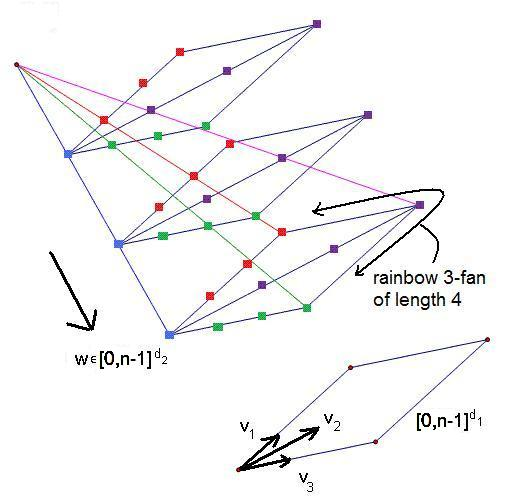
\includegraphics{cnt-chapters/hales-jewett}
\end{figure}

Now for each $x_2$ we have the following pieces of data.
\begin{enumerate}
\item
The base $a_1$ and vectors $v_1,\ldots, v_{m-1}$ in $[0,n-1]^{d_1}$ as defined above: There are at most $(n^{d_1})^m$ possibilities for these.
\item
The colors $C, C_i$ of the base $a_1$ and the sticks $a_1+[1,n-1]v_i,1\leq i\leq m-1$: There are at most $c^m$ choices for these colors.
\end{enumerate}
Hence there are at most $c^mn^{d_1m}$ possibilities for the combined data. Color the points of $[0,n-1]^{d_2}$ with $c^mn^{d_1m}$ colors based on the associated data. 

By the choice of $d_2$, there is a stick of length $n-1$, say (by shifting as in part 1) $a_2+[1,n-1]w$.  
Let the common data for the $n-1$ points in the bar $a_2+[1,n-1]w$ be $a_1,v_1,\ldots, v_{m-1}, C, C_1,\ldots, C_{m-1}$. Now let $a=(a_1,a_2)$; extend the vectors $v_i$ in the $v$-direction by setting $w_i=(v_i,w)$, and include the additional vector $w_m=(0,w)$. See the picture.

We claim that $(a,w_1,\ldots, w_m)$ is a rainbow $m$-fan of length $n$ (in the original coloring). Indeed, the stick $a+[1,n-1]w_i=(a_1,a_2)+[1,n-1](v_i,w)$ has the color $C_i$, the color of corresponding stick in the common cross section. Furthermore, the color of $a+[1,n-1]w_m=a+[1,n-1](0,w)$ is just $C$, the color of the base of the common fan in the cross sections, which is different from the colors $C_1,\ldots, C_{m-1}$. Hence we get a rainbow $m$-fan of length $n$, as needed, completing the induction step.
\end{enumerate}
\end{proof}
It is an interesting exercise to find an explicit value of $N$ that works in Van der Waerden's Theorem by following the above argument.\\

{\Large Problems 4}
\begin{enumerate}
\item If the nonnegative integers are colored with a finite number of colors, does there necessarily exist an infinite monochromatic arithmetic sequence?
\item (HMMT 2009) Find the smallest number of colors needed to color the nonnegative integers so that $a,b$ have different colors whenever $|a-b|$ is a power of 2.
\item (UM 2006) Each positive integer is assigned one of three colors. Show that there exist distinct positive integers $x,y$ such that $x$ and $y$ have the same color and $|x-y|$ is a perfect square.
\item (IMO 1978/6) An international society has members from six different countries. The list of members contains 1978 names, numbered $1,2,\ldots, 1978$. Prove that there is at least one member whose number is the sum of the numbers of two members, not necessarily distinct, of his or her own country.
\item (ISL 1999/C6) Suppose that every integer has been given one of the colors red, blue, green, yellow. Let $x$ and $y$ be odd integers such that $x\neq y$. Show that there are two integers of the same color whose difference is one of the following values: $x,y,x+y,x-y$.
\item (ISL 1995/N7) Does there exist an integer $n>1$ that satisfies the following condition?

The set of positive integers can be partitioned into $n$ nonempty subsets such that an arbitrary sum of $n-1$ integers, one taken from each of any $n-1$ of the subsets, lies in the remaining subset.
\item (ISL 1999/A4) Prove that the set of positive integers cannot be partitioned into three nonempty subsets such that for any two integers $x,y$ taken from two different subsets, the number $x^2-xy+y^2$ belongs to the third subset.
\item (Gallai's Theorem) Given $k,d,c\geq 1$ and $v_1,\ldots, v_k\in \Z^d$, prove that there exists $N$ such that when the points of $[1,N]^d$ are colored with $c$ colors, there exist $x$ and $r\in \Z-\{0\}$ such that $x+rv_1,\ldots, x+rv_k$ all have the same color. 
\end{enumerate}